\documentclass[../main.tex]{subfiles}
\graphicspath{{\subfix{../images/}}}
\begin{document}

Segundo \cite{biazon2017profundezas}, os oceanos representam cerca de 70\% da superfície terrestre na atualidade, mas apesar da sua vasta ocupação, somente 5\% do território oceânico é conhecido pelo homem. A lacuna de conhecimento gera uma crescente demanda na indústria por recursos encontrados \textit{offshore}, como petróleo, recursos minerais (óleos, gás e metais) e biodiversidades.

A indústria apresenta uma crescente expansão em relação ao oceano. No relatório anual de sustentabilidade \cite{petrobras2024} é relatado que 98\% da produção do ano de 2024 veio de águas profundas ou ultraprofundas. Esse cenário de exploração crescente cria uma demanda cada vez maior por tecnologias e mão de obra especializada.

Mergulhadores são uma mão de obra especializada amplamente utilizada na indústria para trabalhos \textit{offshore}, seja para manutenção ou instalação de equipamentos. Segundo \cite{OSHA2023}, a organização de trabalho americana, os perigos enfrentados por profissionais do mergulho incluem afogamento, riscos respiratórios e cardiovasculares, hipotermia e riscos físicos devido ao manuseio de equipamentos pesados embaixo d'água, além dos riscos relacionados a descompressão e possíveis acidentes causados pelo ambiente  de alto risco e nível elevado de estresse.

Dessa maneira, a indústria está constantemente em busca de melhorar a segurança no trabalho. Dentro desse contexto surgem os ROVs (\textit{Remotely Operated Vehicles}), sendo esses uma alternativa estratégica para retirar o trabalhador de uma zona eminente de perigo.

ROVs são veículos subaquáticos que variam de tamanho, podendo ser de maior ou menor porte, e possuem a capacidade de se autopropulsionar abaixo da superfície da água, podendo, em alguns casos, também operar na superfície, dependendo de seu projeto e aplicação. Por serem veículos remotamente operados, podem ser utilizados em aplicações em alta profundidade de forma mais segura por não precisarem da presença de um ser humano na área de perigo. 

Ao tirar o ser humano da zona de perigo são reduzidos os riscos fatais, além de oferecer vantagens operacionais como a possibilidade de um trabalho submerso contínuo e prolongado.

Apesar da utilização de ROVs ser vantajosa e funcional, em relação a utilização de mergulhadores humanos, a operação desses veículos é um desafio devido aos disturbios ambientais constantes gerados pelos oceanos, que contam com correntes marítimas imprevisíveis, baixa visibilidade, entre outras adversidades. 

Assim, para lidar com as adversidades enfrentadas no ambiente subaquático, os ROVs necessitam de sistemas de controle capazes de compensar os ruídos gerados pelas perturbações ambientais, garantindo estabilidade e execução adequada das atividades para as quais foram projetados.

Em \cite{8559384} são citados alguns tipos de controladores, entre eles o controlador PID, caracterizado por ser um controlador simples e amplamente utilizado, é um controle de resposta de velocidade, com efeito linear. Apesar de ser amplamente utilizado, não é o ideal para processos complexos e não lineares ou variantes no tempo.

As redes neurais também são apontadas como um possível controlador para um ROV, sendo essas caracterizadas por serem capazes de aproximar qualquer função não linear na teoria. Apresentam uma alta capacidade de processamento paralelo, o que gera uma grande tolerância a falhas e eficiência no tratamento de múltiplos sinais de entrada e saída. 

Apesar das inúmeras vantagens, é necessário ter cautela pois há a tendência de convergir para mínimos locais, além de sofrer com a lentidão na aprendizagem, limitação no número de camadas e riscos de overfitting. 

Por último é mencionado o controlador fuzzy. Esse controlador é caracterizado por sua independência de uma modelagem matemática exata do objeto de controle, tendo sua essência em estratégias de autocontrole. A lógica fuzzy é capaz de lidar com sistemas não lineares e variantes no tempo, além de ser robusta a ruídos e perturbações externas.

%O foco deste trabalho está em veículos submersos, mais especificamente em ROVs (Remotely Operated Vehicles). 
%Por se tratar de veículos teleoperados, a operação dos ROVs apresenta diversos desafios, como perda de comunicação e falhas em equipamentos cruciais para seu funcionamento. 
%Diante disso, torna-se necessário o desenvolvimento de técnicas capazes de lidar com as adversidades que surgem durante a operação, especialmente em situações em que o ROV não pode ser facilmente recuperado.

Thrusters são dispositivos responsáveis por impulsionar a embarcação, ou seja, são os propulsores que garantem sua movimentação. 

Um dos desafios enfrentados por veículos que utilizam thrusters é a possibilidade de falha em um ou mais desses dispositivos durante a operação, o que levanta a questão de como recuperar o controle do veículo ou garantir que ele continue navegando mesmo diante dessas falhas.

Dessa forma, o objetivo principal deste trabalho é abordar o problema da falha de thrusters através da otimização e redistribuição das forças restantes pós-falha, buscando manter a estabilidade e a funcionalidade do sistema mesmo em condições adversas.

Os estudos relacionados a otimização serão aplicados ao robô BlueROV, um veículo subaquático do tipo ROV desenvolvido pela empresa BlueRobotics. A Figura~\ref{rov_view} apresenta uma representação visual do robô.

\begin{figure}[!htb]
  \centering
  \caption{Vistas frontal, lateral, isométrica e inferior do robô BlueROV.}
  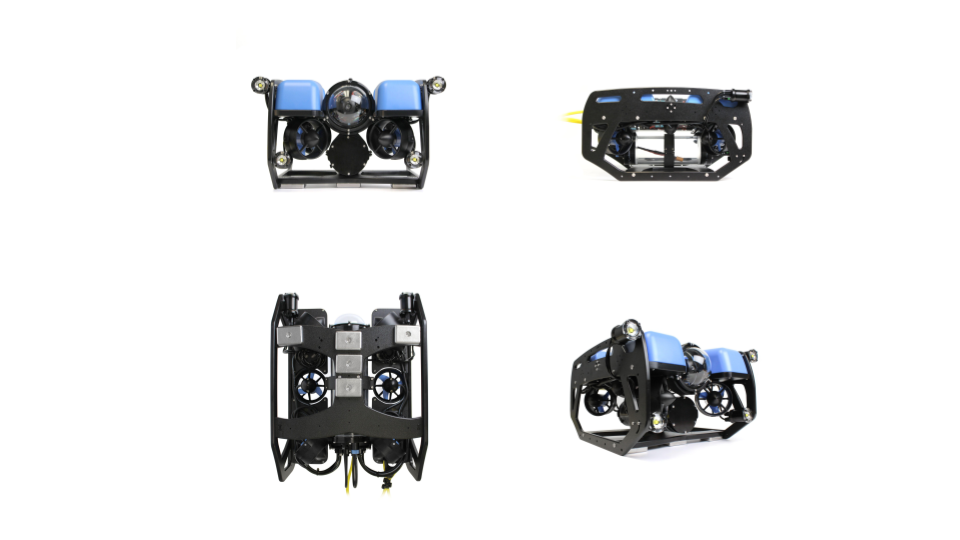
\includegraphics[width=0.45\textwidth]{images/vistas_bluerov (1) .png}
  \vfill
  Fonte: Autores.
  % \vspace{-\baselineskip}
  \label{rov_view}
\end{figure}

A modelagem do sistema de controle será desenvolvida levando em consideração as dimensões, características e requisitos específicos do BlueROV. 

Todos os testes e simulações serão realizados em ambiente computacional, utilizando ferramentas como o Gazebo, para simular a movimentação do ROV pré e pós-falha, para a observabilidade da realocação das forças otimizadas.

\end{document}
